\chapter{Introduction}

Over the past decade, Virtual Reality (VR) technology has experienced a resurgence in popularity due to the development of a number of affordable, consumer-quality head-mounted displays\footnote{The price of a consumer-quality VR headset is between approximately 20 and 1000 USD as of January 2021, including headsets for use with a smartphone. \\(\url{https://www.tomsguide.com/us/best-vr-headsets,review-3550.html}, \emph{accessed Jan 13, 2021})}. These displays allow a user to experience and interact with a virtual environment in 3D, for example by playing games, or by taking virtual tours of cities, historical landmarks, or remote locations in nature.
%\footnote{``10 of the best virtual reality travel experiences'', Paul Joseph, Travelmag (\url{https://www.travelmag.com/articles/virtual-reality-travel-experiences/}, \emph{accessed Jan 13, 2021})}

Some of these environments are modeled meticulously in 3D, while others use 360\degree images taken on location. Often, the 3D-modeled environments allow a lot of freedom of movement, enabling users to ``walk'' around and inspect elements of the scene at will. Unfortunately, modeling a real environment by hand to be viewed interactively requires an enormous amount of time and effort, and even then it is very difficult to achieve photo-realism. An alternative is to capture the location with a 360\degree camera, which records all of the surroundings in a single image. Viewing these images offers photo-realism (as they are actual photos), but often unnatural navigation, for example forcing the user to ``jump'' from one image location to the next, instead of being able to ``walk'' smoothly around the scene. Nevertheless, the ease of capturing 360\degree images with modern 360\degree cameras, along with the significant advantage of providing photo-realism, makes this an attractive method for creating immersive VR environments.

The difficulties of navigating an environment captured through 360\degree cameras are not a new phenomenon. Such problems are also relevant in virtual tours that exist outside of the realm of VR, viewed on regular computer or smartphone screens, for example interactive tours of museums, real-estate, or other locations of interest. A prominent example is Google's Street View, which allows users to navigate streets and monuments around the world by way of 360\degree images.

Whether a scene is viewed stereoscopically with a head-mounted display, or monoscopically on a flat screen, a significant obstacle at the moment is the problem of interactive, user-driven navigation. Ideally, a user would be able to go anywhere they liked in the scene, and view anything they wanted from any angle and at any level of detail. Unfortunately, for environments captured by way of a 360\degree camera, this type of interaction would require a prohibitive amount of data, as well as being impossible to manually execute, since a separate image would have to be captured at every possible viewing position.
\newpage

An alternative to capturing all of these viewpoints manually is to generate them digitally. This requires capturing a much smaller subset of images and using these to generate the desired, novel viewpoints. Generating new images based on already captured images is generally known as \emph{image-based rendering} (IBR), or \emph{image-based synthesis}. There are many different approaches to synthesizing new images from captured ones, and they can generally be categorized in two different ways:
%These approaches can be divided into general categories which can be defined by \ldots
\begin{itemize}
  \item by the spacial limitations imposed by the synthesis technique, including degrees of freedom and range of motion
  \item by the type and amount of information extracted from the captured images
\end{itemize}
%the area where new images can be synthesized, as well as the type and amount of information extracted from the captured images.
%degrees of freedom (DoF) that the technique can synthesize images with

\noindent
The area and the degrees of freedom (DoF) required for navigation usually depend on the goal and requirements of the application: A virtual tour on a pre-defined path for example, would only require generating intermediate views between existing viewpoints (i.e.\ synthesis with 1-DoF) for a smooth transition. For a less constrained virtual tour that enables users to navigate freely on a plane, generating viewpoints with 2-DoF at eye-level could be sufficient. Users could move around and look in any direction but not change their viewing height. Some applications may require 3-DoF, for example in order to enable users to closely inspect certain objects from all angles, but restrict them from moving away from the object.

Depending on the type of scene, the required fidelity, and the real-time requirements, different IBR techniques leverage different amounts and types of information extracted from the input images.
For example, there are approaches that extract as much geometry information as possible from the set of images and try to reconstruct the 3D geometry of the scene as closely as possible. These approaches can suffer from the problem of extracting accurate geometry information, since errors in geometry can lead to unappealing results.
Other approaches try to extract some information from the image, such as feature correspondences, or motion vectors (optical flow), which enables interpolation between pairs of images, i.e.\ a smooth transition with 1-DoF.
Finally, there are approaches that use no semantic image information whatsoever. Instead, they may use color values, simple proxies for the scene geometry, or information about the relative location of captures, but they tend to operate on a pixel level. Although there is no specific label for this kind of synthesis, for the purpose of this thesis, it will be referred to as \emph{pixel-based synthesis}.

One very basic form of pixel-based synthesis is to use a simple proxy (``stand-in'') geometry, for example a sphere, in place of the real scene geometry\footnotemark. This allows for resampling the captured images in order to create a new viewpoint at any location within the scene, without having to estimate or record the actual scene geometry. However, a significant difference between the proxy and the actual geometry can lead to severe distortions and artefacts in the resampled images. Although this basic form of pixel-based rendering using proxy geometry may be unsuitable for scenes where the real geometry differs greatly from the proxy geometry, it may be possible to improve these results by combining the basic technique with a 1-DoF interpolation method.
\footnotetext{The term ``proxy geometry'' is used in this thesis as a term for the model used in place of the real scene geometry. It can be anything from a simple geometric shape such as a sphere, to a simplified version of the real scene geometry}


\section*{Problem Statement}
A number of 1-DoF interpolation techniques exist, many of which use some form of feature correspondence. Flow-based interpolation is one of these techniques that has already been used successfully for 360\degree images. It uses motion vectors (``optical flow'') between pairs of images to interpolate new viewpoints between them. The goal of this thesis is to answer the following research questions:

\begin{enumerate}
  \item Can flow-based interpolation be used in pixel-based 2-DoF synthesis with proxy geometry?
  \item If it can, does the flow-based interpolation improve the accuracy of the results compared to the basic pixel-based synthesis?
\end{enumerate}

In order to measure the accuracy of the different results, the synthesized images are compared with the ground truth images using two different error metrics, as well as being assessed visually.


\section*{Methodology}
%In order to implement and evaluate an algorithm that combines basic pixel-based synthesis and flow-based interpolation, this thesis follows an approach consisting of two distinct phases: implementation and evaluation (Figure~\ref{fig:methodology}). The implementation consists of first developing a basic pixel-based synthesis algorithm using proxy geometry. Then, based on existing 1-DoF flow-based interpolation algorithms (presented in Section~\ref{sec:related_work}), the extended pixel-based algorithm using flow-based interpolation is developed. The approach and implementation are presented in Chapter~\ref{chap:implementation}.
%
%The evaluation is used to judge under which circumstances the flow-based algorithm yields more accurate results than the basic pixel-based algorithm.
%The evaluation step is further divided into three phases. In the preparation phase, based on the parameter space described in detail in Section~\ref{sec:params}, data for testing and evaluation is acquired, including virtual and real scenes. Additionally, the error metrics are adapted for 360\degree images (Section~\ref{sec:eval_methodology}).
%Then, in the synthesis and testing phase, the images are synthesized using the implementations developed in the implementations step. Using the result images and the ground truth data generated during the data acquisition, error calculation is performed with the adapted metrics.
%Finally, using the calculated error values, along with the synthesized images, the results are analyzed.
%The analysis is made up of two parts: First, an more extensive analysis is performed on the virtual data that explores the chosen parameters (Section~\ref{sec:limit_eval}). Then, the results using the real data are examined as a proof-of-concept (Section~\ref{sec:pof_eval}). 

The methodical approach used in this thesis consists of two distinct phases which address the two research questions: The first phase (the ``implementation phase'') aims to design and implement a pixel-based 2-DoF synthesis with proxy geometry using flow-based interpolation. The second phase (the ``evaluation phase'') aims to examine whether the flow-based interpolation can improve the results of the basic synthesis without flow-based interpolation. Figure~\ref{fig:methodology} shows the details of the methodical approach, including these two phases, along with the inputs and the results of the process.

For the implementation phase, first, a basic pixel-based synthesis algorithm using proxy geometry is developed (``synthesis with regular blending''). Then, the basic synthesis is combined with an existing flow-based interpolation algorithm (the input to the implementation phase in Figure~\ref{fig:methodology}) to create a flow-based synthesis algorithm (``synthesis with flow-based blending''). The development of this proof-of-concept algorithm proves that it is possible to leverage flow-based interpolation for pixel-based 2-DoF synthesis with proxy geometry, which is the first result.

The algorithms developed in the implementation phase are then tested and evaluated in the evaluation phase.
%The goal of this phase is to determine the effect of the chosen parameters on the results, as well as to examine under which circumstances the synthesis with flow-based blending performs better than the synthesis with regular blending. The ``performance'' is defined as the accuracy of the results compared to ground truth data and is measured using mathematical error metrics that are adapted for 360\degree images.
The evaluation phase is further divided into three steps, separated vertically in Figure~\ref{fig:methodology}: preparation, synthesis and testing, and evaluation. In the preparation step, data for testing and evaluation is acquired based on the defined parameter space, including virtual and real scenes. Then, the images are synthesized with both the regular blending and the flow-based blending algorithm, which are the output of the implementation phase. The resulting images are then compared with the ground truth data using the error metrics adapted for 360\degree images. 
Finally, using the calculated error values, along with the synthesized images, the results are analyzed, leading to the conclusion that the synthesis using flow-based blending performs better than the synthesis using regular blending in a number of cases, particularly when the regular blending produces significant artefacts. This full evaluation is the second result of the thesis.

\begin{figure}
		\centering
		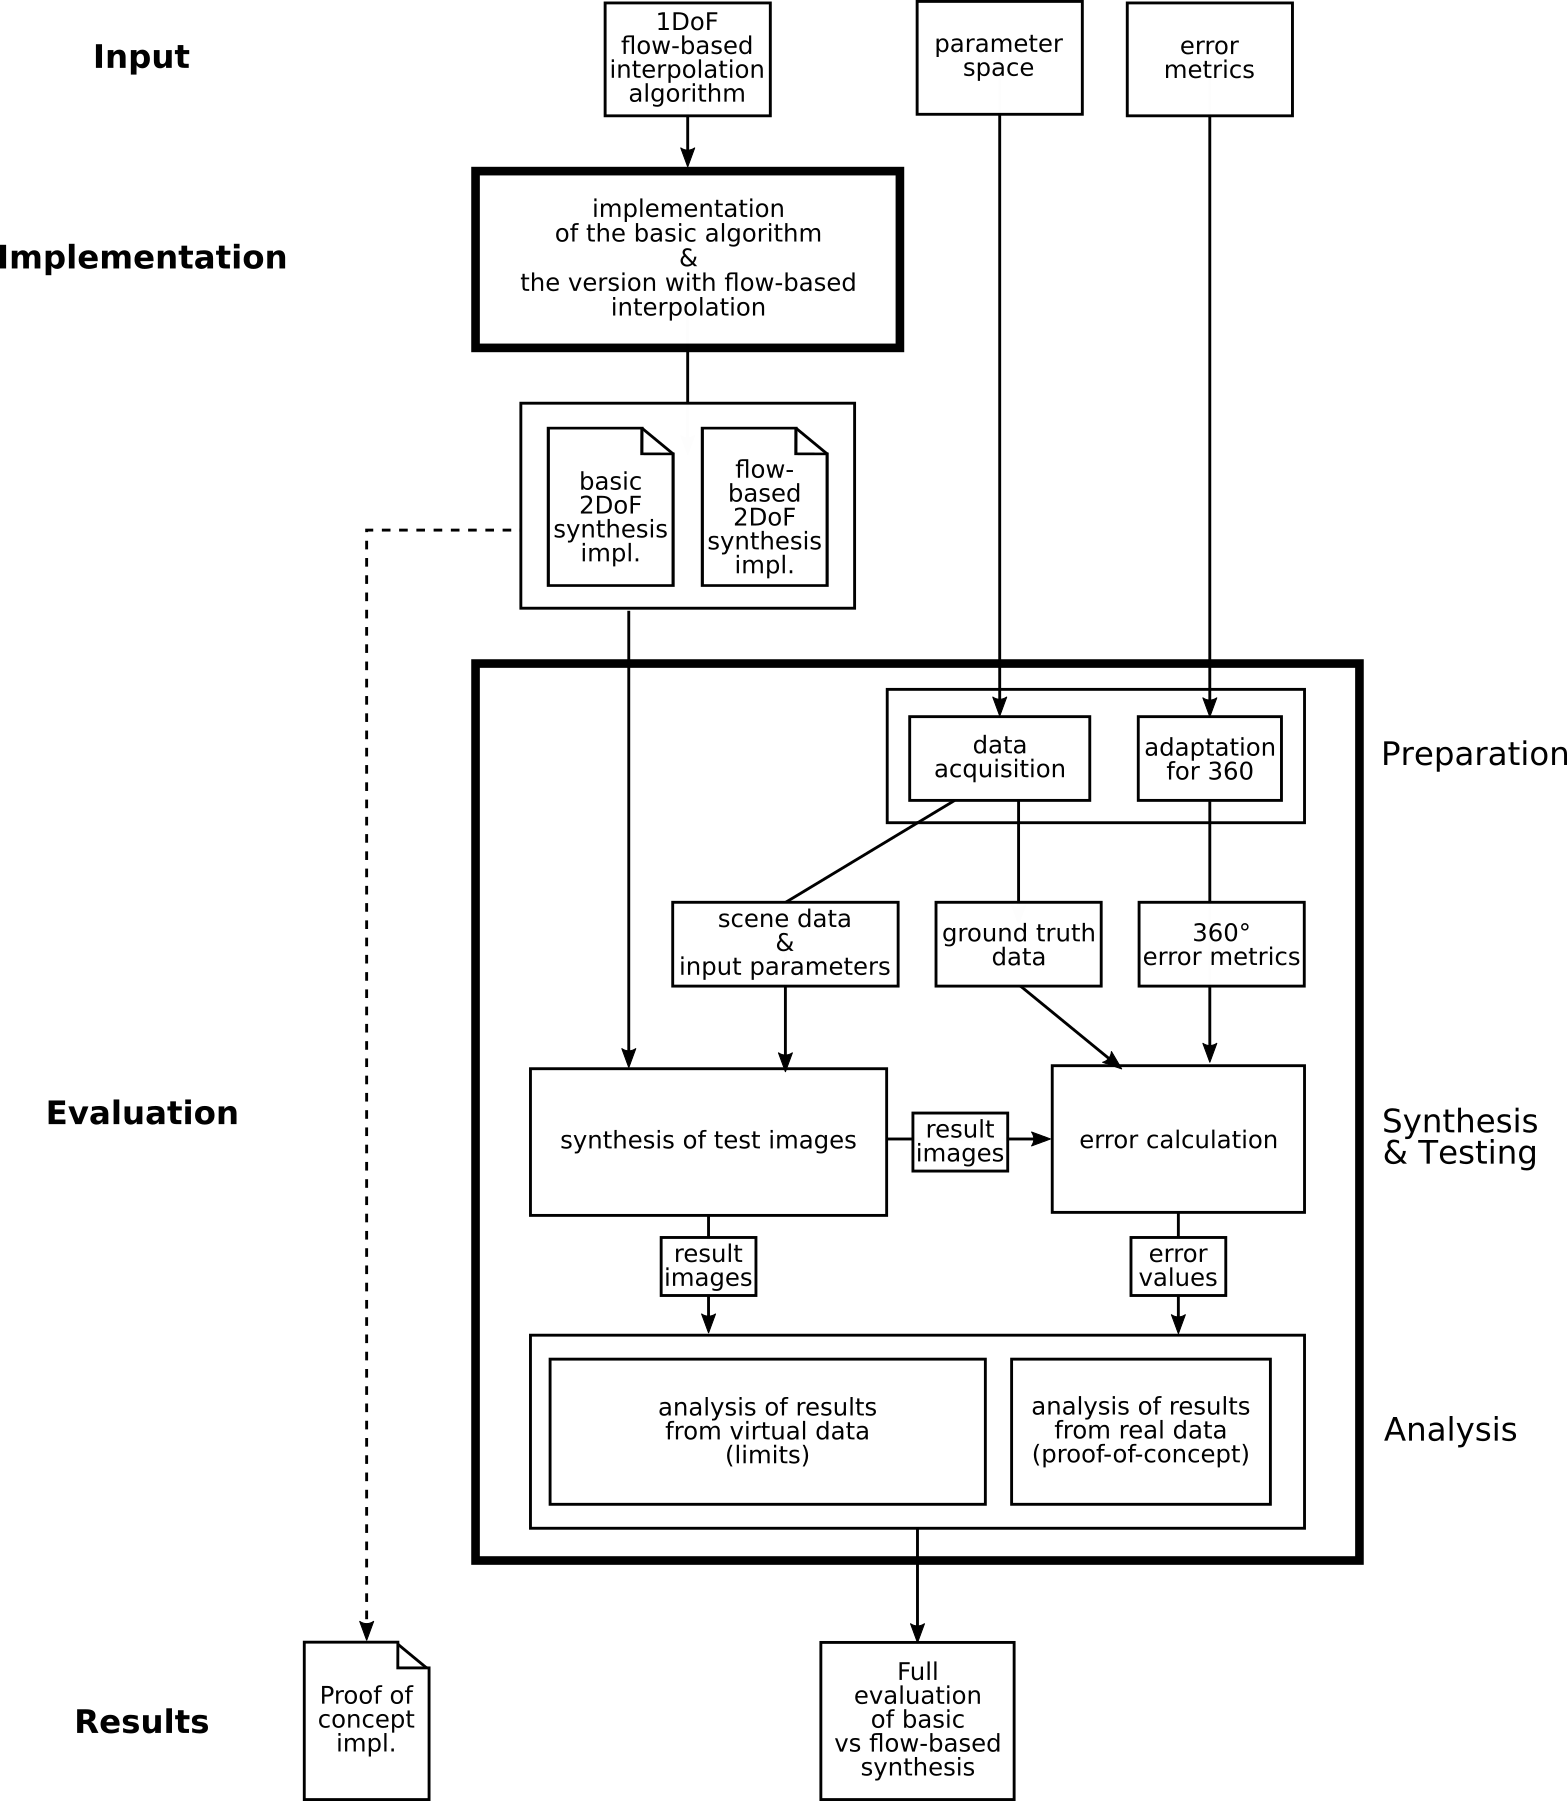
\includegraphics[width=0.9\textwidth]{01/methodology.png}
		\caption{Methodical approach}
		\label{fig:methodology}
\end{figure}


\section*{Scope}
As the number of possible different environments is infinite, as well as the positions at which images can be captured, it is necessary to limit the parameter space for testing and evaluation. First of all, only indoor scenes are examined. The scenes are assumed to be static, meaning the objects within the scene do not change their positions. To reduce the complexity of the implementation, as well as the number of necessary input images to be captured, only 2-DoF synthesis is considered. Specifically, all captured and synthesized viewpoints are located on a plane at approximate eye-level parallel to the ground. 

\noindent
The parameters that will be examined in detail are:
\begin{description}
  \item[Difference between the scene geometry and the proxy geometry] The proxy geometry used in this thesis is a sphere of the approximate size of the scene. Scenes of different basic shapes, containing different objects, are tested in order to gauge the effect of the difference between the proxy geometry and the scene.
  \item[Density of captured viewpoints] The density of the captured viewpoints is an important aspect, as it is directly related to the effort required to capture a scene (the higher the necessary density, the more images need to be captured). In order to assess the effect of different densities on the accuracy of the results, different densities of captured viewpoints are tested.
    %For the evaluation in this thesis, the viewpoints used for synthesis (the ``captured viewpoints'') are arranged on a regular grid. The effect of different densities on the accuracy of the results is explored, specifically, grids of between 3m and 30cm distance are used.
  \item[Position of synthesized points relative to captured points] A synthesized viewpoint can theoretically be located anywhere within the boundaries of the scene, as long as it is at the defined eye-level. The relative position of the synthesized point to the captured points is likely to have an effect on the accuracy of the result and will be examined in more detail by synthesizing a dense grid of viewpoints within a scene.
    %This means that it can be very close to a captured viewpoint, or further away. Furthermore, it may make a difference whether the synthesized viewpoint is directly on a line between captured viewpoints. A dense grid of viewpoints is synthesized to test the effect of the relative positioning.
\end{description}

\noindent
These parameters will not be examined exhaustively, as this is impossible, given the infinite possibilities of scene shapes and object placements, alone. Instead, for each parameter to be examined, a scenario is designed that tests this parameter in a reasonable context.

%Since the implementation is a basic proof-of-concept, a user study does not make much sense, since the results are expected to have some distinct artefacts. Instead, two mathematical error metrics are used to compare the 

%2-DoF synthesis without geometry in indoor environments
%variable
%quantified:
%  the location of synthesized points relative to the captured points
%  density of captured viewpoints
%
%not quantified
%  effect of objects within the scene
%  scene - model difference
%  the location of synthesized points within the scene (near walls, objects, etc)
%
%  evaluation:
%    mathematical error metrics to compare result to ground truth: mean absolute error and ssim
%
%basic proof of concept implementation \ar not perfect, real-time
%not an exhaustive evaluation of all possible parameters \& combinations
%not a comparison to other implementations (missing benchmark data and implementation of other methods is outside of scope)
%
%will be evaluating following scenarios:
%Effect of Viewpoint Density
%Viewpoint Density and Choice of Viewpoints to be Synthesized
%Position of Synthesized Viewpoints Relative to Captured Viewpoints
%Effect of Different Scenes


\section*{Contributions}
The contributions of this thesis are:
\begin{itemize}
  \item An algorithm for pixel-based 2-DoF synthesis algorithm with flow-based interpolation (``synthesis with flow-based blending'')
  \item A basic proof-of-concept implementation of this algorithm
  \item An evaluation of the results of this algorithm, including a comparison with the results of the algorithm with regular blending
\end{itemize}

\noindent
The results show that in the majority of cases where the basic method with regular blending produces significant artefacts, the synthesis using flow-based blending does improve the the accuracy of the results. 

%The results of this thesis can be the basis of various future work. Since the implementation is a first attempt at combining the two methods, the problems and limitations discovered in the evaluation can be used to improve future versions. Alternative proxy geometries could be examined, potentially based on sparse scene geometry, which would improve the basic results and could lead to a distinct improvement of the flow-based results. Furthermore, parallelization and optimization could be used in order to achieve real-time framerates. 


\section*{Outline}
In order to understand the underlying concepts and techniques that are used in the synthesis approach proposed in this thesis, Section~\ref{sec:fundamentals} introduces the fundamentals of 360\degree images and optical flow, followed by related work in the field of image-based synthesis in Section~\ref{sec:related_work}.
Based on this information, Section~\ref{chap:implementation} presents the approach and implementation details of the pixel-based 2-DoF synthesis algorithm with regular blending and flow-based blending.
Then, in order to understand how the algorithm is evaluated, the evaluation parameters and methodology are presented in Section~\ref{sec:params} and Section~\ref{sec:eval_methodology}, followed by the evaluation of the virtual scenes based on the selected parameters in Section~\ref{sec:limit_eval} and the proof-of-concept evaluation of the real scene in Section~\ref{sec:pof_eval}. Based on the results of these evaluations, the limitations of the evaluation are discussed in Section~\ref{sec:limitations}.
Finally, building on the insights gained in the evaluation, possibilities for future work are presented in Section~\ref{chap:conclusion}, along with the conclusion of the thesis.

%The structure of this thesis follows the order presented in the methodical approach:
%First, the underlying concepts of 360\degree images and optical flow are presented (Section~\ref{sec:fundamentals}), along with related work in the field of image-based synthesis (Section~\ref{sec:related_work}). Next, the ``interpolation step'' is presented, including the approach to the pixel-based 2-DoF synthesis algorithm with regular blending and flow-based blending (Section~\ref{sec:approach}) along with the details of the implementation (Section~\ref{sec:impl_details}).
%For the ``evaluation step'', first the evaluation parameters and methodology are presented (Section~\ref{sec:params} and Section~\ref{sec:eval_methodology}), followed by the evaluation of the virtual scenes (Section~\ref{sec:limit_eval}) and the real scene (Section~\ref{sec:pof_eval}). Based on the insights gained in these evaluations, the limitations of the evaluation are discussed (Section~\ref{sec:limitations}).
%Finally, possibilities for future work are presented, along the conclusion of the thesis (Section~\ref{chap:conclusion}).

